% !TeX spellcheck = en_US
\newpage
\section{Moving Bitmaps}\index{Bitmap!moving}
\subsection{Class \texttt{Rect}/\texttt{FRect}}
 In the summary of the previous chapter, we noted that when displaying bitmaps we need the \emph{upper-left corner} as the position value, and we need the \emph{height} and \emph{width}, for example for distance calculations. These values can be conveniently encoded in a rectangle. For this purpose, Pygame provides the classes \texttt{pygame.rect.Rect}\myindex{pyg}{\texttt{rect}!\texttt{Rect}|underline}\randnotiz{Rect} (integers only) and \texttt{pygame.rect.FRect}\myindex{pyg}{\texttt{rect}!\texttt{FRect}|underline}\randnotiz{FRect} (floating-point numbers). In \abbref[vref]{picRect01}, you can find what I consider to be the most important attributes of this class.

\begin{figure}[H]
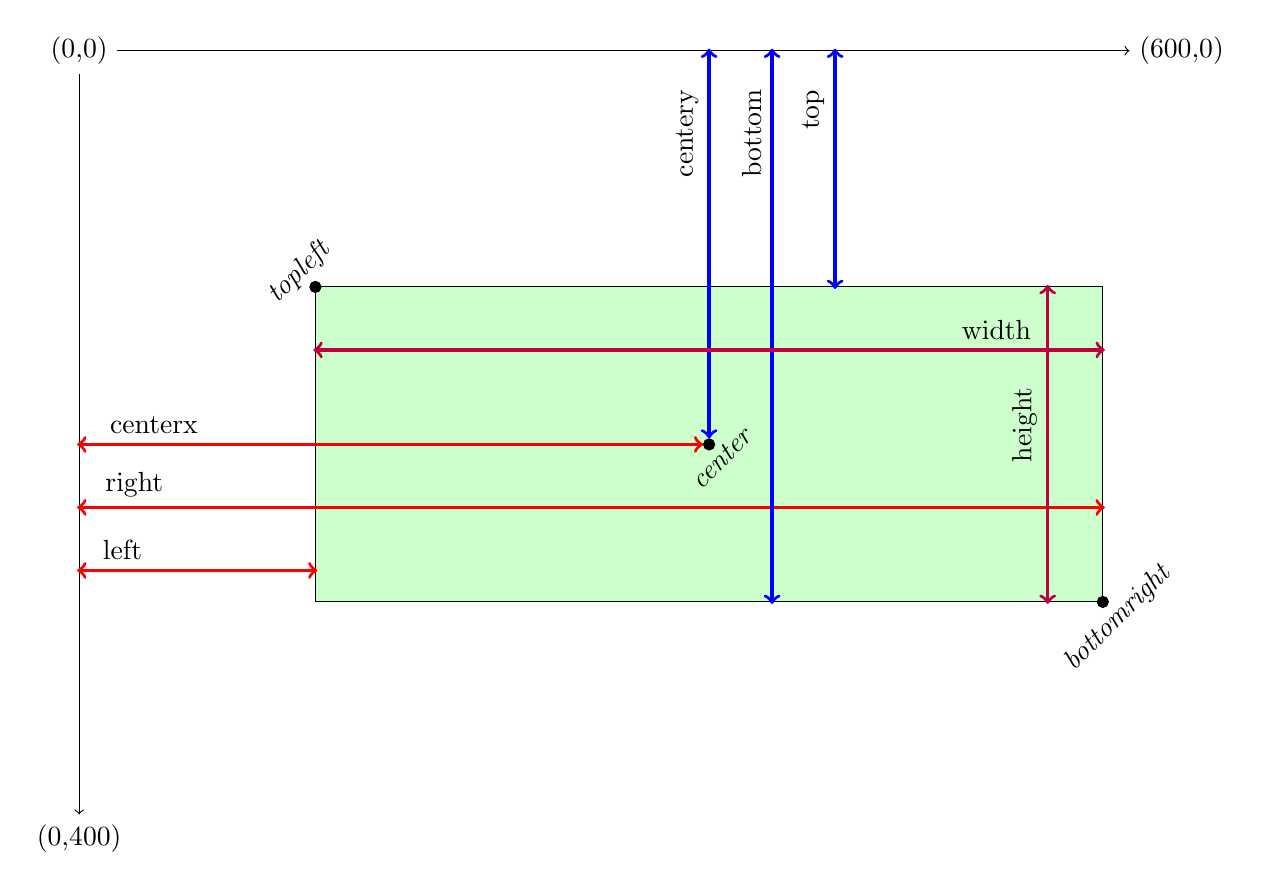
\begin{tikzpicture}
%Bildschirm Koordinatensystem
\draw
 (0,10) node (o) {(0,0)}
 (0,0) node (y) {(0,400)}
 (14,10) node (x) {(600,0)}
;
\draw[->] (o) -- (x);
\draw[->] (o) -- (y);

%Rechteck
\draw
 (3,7) node (topleft) {}
 (13,3) node (bottomright) {}
 (8.0,5) node (centerxy) {}
;
\filldraw[fill=green!20] (topleft) rectangle (bottomright);
\draw (topleft) node[above, rotate=45] {\emph{topleft}};
\draw (bottomright) node[below, rotate=45] {\emph{bottomright}};
\filldraw[fill=black] (centerxy) circle (2pt) node[below, rotate=45] {\emph{center}};
\filldraw[fill=black] (topleft) circle (2pt);
\filldraw[fill=black] (bottomright) circle (2pt);

%Left
\draw
 (-0.15,3.4) node (left1) {}
 (3.15,3.4) node (left2) {}
;
\draw[<->, very thick, red] (left1) -- (left2) node[above, black, xshift=-2.6cm] {left};


%Right
\draw
 (-0.15,4.2) node (right1) {}
 (13.15,4.2) node (right2) {}
;
\draw[<->, very thick, red] (right1) -- (right2) node[above, black, xshift=-12.45cm] {right};

%Centerx
\draw
 (-0.15,5.0) node (cx1) {}
 (8.05,5.0) node (cx2) {}
;
\draw[<->, very thick, red] (cx1) -- (cx2) node[above, black, xshift=-7.1cm] {centerx};

%top
\draw
 (9.6,10.15) node (top1) {}
 (9.6,6.85) node (top2) {}
;
\draw[<->, very thick, blue] (top1) -- (top2) node[above, black, yshift=2.4cm, rotate=90] {top};

%bottom
\draw
 (8.8,10.15) node (bottom1) {}
 (8.8,2.85) node (bottom2) {}
;
\draw[<->, very thick, blue] (bottom1) -- (bottom2) node[above, black, yshift=6.1cm, rotate=90] {bottom};

%Centery
\draw
 (8.0,10.15) node (cy1) {}
 (8.0,4.95) node (cy2) {}
;
\draw[<->, very thick, blue] (cy1) -- (cy2) node[above, black, yshift=4cm, rotate=90] {centery};

%Width
\draw
 (2.85,6.2) node (w1) {}
 (13.15,6.2) node (w2) {}
;
\draw[<->, very thick, purple] (w1) -- (w2) node[above, black, xshift=-1.5cm] {width};

%height
\draw
 (12.3,7.15) node (h1) {}
 (12.3,2.85) node (h2) {}
;
\draw[<->, very thick, purple] (h1) -- (h2) node[above, black, yshift=2.4cm, rotate=90] {height};

\end{tikzpicture}
\caption{Elements of a \texttt{Rect}-Object}\label{picRect01}
\end{figure}

\myindex{pyg}{\texttt{rect}!\texttt{Rect}!\texttt{centerx}}%
\myindex{pyg}{\texttt{rect}!\texttt{Rect}!\texttt{right}}%
\myindex{pyg}{\texttt{rect}!\texttt{Rect}!\texttt{left}|underline}%
\myindex{pyg}{\texttt{rect}!\texttt{Rect}!\texttt{centery}}%
\myindex{pyg}{\texttt{rect}!\texttt{Rect}!\texttt{bottom}}%
\myindex{pyg}{\texttt{rect}!\texttt{Rect}!\texttt{top}|underline}%
\myindex{pyg}{\texttt{rect}!\texttt{Rect}!\texttt{topleft}}%
\myindex{pyg}{\texttt{rect}!\texttt{Rect}!\texttt{bottomright}}%
\myindex{pyg}{\texttt{rect}!\texttt{Rect}!\texttt{center}|underline}%
\myindex{pyg}{\texttt{rect}!\texttt{Rect}!\texttt{width}|underline}%
\myindex{pyg}{\texttt{rect}!\texttt{Rect}!\texttt{height}|underline}%
\myindex{pyg}{\texttt{rect}!\texttt{Rect}!\texttt{size}|underline}%

\myindex{pyg}{\texttt{rect}!\texttt{FRect}!\texttt{centerx}}%
\myindex{pyg}{\texttt{rect}!\texttt{FRect}!\texttt{right}}%
\myindex{pyg}{\texttt{rect}!\texttt{FRect}!\texttt{left}|underline}%
\myindex{pyg}{\texttt{rect}!\texttt{FRect}!\texttt{centery}}%
\myindex{pyg}{\texttt{rect}!\texttt{FRect}!\texttt{bottom}}%
\myindex{pyg}{\texttt{rect}!\texttt{FRect}!\texttt{top}|underline}%
\myindex{pyg}{\texttt{rect}!\texttt{FRect}!\texttt{topleft}}%
\myindex{pyg}{\texttt{rect}!\texttt{FRect}!\texttt{bottomright}}%
\myindex{pyg}{\texttt{rect}!\texttt{FRect}!\texttt{center}|underline}%
\myindex{pyg}{\texttt{rect}!\texttt{FRect}!\texttt{width}|underline}%
\myindex{pyg}{\texttt{rect}!\texttt{FRect}!\texttt{height}|underline}%
\myindex{pyg}{\texttt{rect}!\texttt{FRect}!\texttt{size}|underline}%

In the figure, line segments are shown in normal font, while points are shown in \textit{italic font}. The segments are one-dimensional, and the points are two-dimensional $(x, y)$. The coordinate~$x$ represents the horizontal distance from the origin of the coordinate system, and~$y$ represents the vertical distance. The meaning of the individual labels should be self-explanatory.

The nice advantage is that all these values are computed from each other. For example, if I set \texttt{topleft = (10, 10)} and \texttt{width, height = 30, 40}, all other values are calculated automatically. I no longer need to compute the right edge manually using \texttt{left + width}; instead, I can directly use \texttt{right}.

It is also often useful to work with the center position \texttt{center} or the corresponding coordinates \texttt{centerx} and \texttt{centery}. If I change the center to \texttt{center = (100, 10)}, all other values are updated accordingly and do not need to be recalculated by me -- very convenient.

Let us take a look at a reduced version of the last source code. In \srcref[vref]{srcInvader05}, the \texttt{Rect} class is already being used. For example, in \zeiref{srcInvader0504a} the window dimensions are stored in a \texttt{Rect} object. 

\lstsource{SRC/00 Introduction/04 Moving/config.py}{1}{999}{python}{Moving Bitmaps: \texttt{config.py}}{srcInvaderConfig00}

As a result, the screen information can be accessed conveniently and without performing manual calculations in \zeiref{srcInvader0504b}, \zeiref{srcInvader0502}, and \zeiref{srcInvader0503}.

\lstsource{SRC/00 Introduction/04 Moving/invader05.py}{6}{36}{python}{Moving Bitmaps, Version 1.0}{srcInvader05}

For \texttt{Surface} objects, we can conveniently create a \texttt{Rect} object using \texttt{pygame.Surface\-.get\-\_rect()}\myindex{pyg}{\texttt{Surface}!\texttt{get\_rect()}}\randnotiz{get\_rect()} (\zeiref{srcInvader0501}). Positioning can now be handled much more easily via the attributes. For example, the center no longer needs to be part of a calculation; instead, I can directly set the horizontal center to half the window width (\zeiref{srcInvader0502}). Likewise, the vertical coordinate no longer has to be considered from the top edge; instead, I can specify the distance of the bottom edge from the screen edge in a much more intuitive way (\zeiref{srcInvader0503}). And as a final bonus, the \texttt{Rect} object can even be passed directly as a parameter to the \texttt{blit()} function\randnotiz{blit()}\myindex{pyg}{\texttt{Surface}!\texttt{blit()}} (\zeiref{srcInvader0504}).

\myebild{invader05.png}{0.8}{Moving Bitmaps, Version 1.0}{picInvader05}

The result is unspectacular (see \abbref[vref]{picInvader05}) and has
nothing to do with movement yet.

\subsection{Introduction}

 Movement in games is animated by changing positions. If the spaceship is supposed to move to the right, the horizontal coordinate of the ship therefore has to increase. Which horizontal coordinate you use for this -- \texttt{left}, \texttt{right}, or \texttt{centerx} -- can be chosen depending on your game logic. In our example, this does not matter, so I will use \texttt{left}.

\lstset{firstnumber=26}
\begin{lstlisting}
defender_rect.left += 1
\end{lstlisting}

This small addition alone now causes our spaceship to move to the right. The \texttt{+1} encodes two pieces of information:

\begin{itemize}
	\item \textbf{Direction:}\randnotiz{Direction}\index{Direction} Here, the sign is \texttt{+}. This increases the value of \texttt{left} in each loop iteration; as a result, the left edge of the graphic moves to the right. If you wanted to move to the left, the sign would have to be	\texttt{-}.	In that case, the horizontal coordinate would become smaller and approach~0. Completely analogously, the sign also controls the direction in the vertical axis.	A \texttt{+} moves the graphic downward, and a \texttt{-} moves it upward.	Try it out!
	
	\item \textbf{Speed:}\randnotiz{Speed}\index{Speed}	The \texttt{1} specifies by how much the value of \texttt{left}	changes. The larger this value is, the larger the jumps between frames;	the movement appears faster.
\end{itemize}


\lstsource{SRC/00 Introduction/04 Moving/invader05b.py}{17}{28}{python}{Moving Bitmaps, Version 1.2}{srcInvader05b}

These two pieces of information are now used in \srcref[vref]{srcInvader05b} to make movement much more flexible. In \zeiref{srcInvader0505}, the speed is now represented by the variable \texttt{defender\_speed}. This would allow us to change the speed dynamically during the game, for example when accelerating by firing rocket thrusters.

The direction is also stored in a variable in \zeiref{srcInvader0506}: \texttt{defender\_direction}. At the moment it is positive, but we will soon see that we can also use it for changing direction.

Both values can now be used in \zeiref{srcInvader0507} to calculate the new horizontal position.

If you run the program, the defender will leave the screen after a while and disappear beyond the right edge, never to be seen again. Let us now use our rectangle for a first simple collision check. I want the spaceship to \emph{bounce} off the edges and reverse its direction.

\lstsource{SRC/00 Introduction/04 Moving/invader05c.py}{27}{32}{python}{Move Bitmaps, Version 1.3}{srcInvader05c}

I hope you can recognize the idea behind the code. After calculating the new horizontal position, \zeiref{srcInvader0508} checks whether the new right edge of the bitmap has reached or exceeded the right edge of the screen. If this is the case, the sign of the direction variable is simply reversed\index{Direction change}\randnotiz{Direction change}! The same logic works analogously when the left edge of the screen is reached.

Try combining this with vertical movement as well.

There is still one problem: In \zeiref{srcInvader0507}, the new position is assigned to the \texttt{Rect} object even though it may already extend beyond the edge. With a speed of \texttt{1} or \texttt{2}, this may not be very noticeable, but if we set the speed to the width of the spaceship, the problem becomes obvious (temporarily set \texttt{cfg.FPS = 5} so that you can see it clearly). The spaceship ends up leaving the screen halfway. 
 
So we should check the new position first and only then assign it to the \texttt{Rect} object \texttt{defender\_rect}. In this context, let us introduce a very useful method of the \texttt{Rect} class: \texttt{pygame.rect.Rect.move()}\myindex{pyg}{\texttt{rect}!\texttt{Rect}!\texttt{move()}|underline}\randnotiz{move()}. 
 
\lstsource{SRC/00 Introduction/04 Moving/invader05d.py}{27}{35}{python}{Move Bitmaps, Version 1.4}{srcInvader05d}

The new function appears for the first time in \zeiref{srcInvader0510}. It takes two parameters. The first one specifies the horizontal displacement, and the second one specifies the vertical displacement. Since we do not want to change the vertical position, this parameter is constant~0 in our example. The function returns a new \texttt{Rect} object containing the updated position values. We store this temporarily in \texttt{newpos}.

The subsequent collision checks are then performed using the \texttt{newpos} rectangle. If a collision occurs, the direction values are changed as before. Likewise, the left edge of the bitmap is aligned with the left edge of the screen, and the right edge is aligned with the right edge. After that, \texttt{newpos} becomes the new rectangle for the defender (\zeiref{srcInvader0511}).


\begin{figure}[H]
\begin{center}
\begin{tikzpicture}
\node (myfirstpic) at (0,0) {\includegraphics[scale=0.8]{invader06.png}};

\draw
 (-1.8cm,-1.3cm) node (a) {}
 (5.8cm,-1.3cm) node (b) {}
 (5.8cm,-0.57cm) node (c) {}
 (3.4cm,-0.57cm) node (d) {}
;
\draw[>->, very thick, red, densely dotted] (a) -- (b) ;
\draw[>->, very thick, red, densely dotted] (c) -- (d) ;

%node[above, black, xshift=-2.6cm] {move left}
%\draw[->] (a) -- (b);
%\draw[->] (o) -- (y);


%Left
%\draw
% (-0.15,3.4) node (left1) {}
% (3.15,3.4) node (left2) {}
%;
%
\end{tikzpicture}
\caption{The Defender moves and bounces}\label{picBewegung01}
\end{center}
\end{figure}

%%%%%%%%%%%%%%%%%%%%%%%%%%%%%%%%%%%%%%%%%%%%%%%%%%%%%%%%%%%%%%%%%%%%%%%%%%%%%%%%
\subsection{More Input}
\subsubsection{Normalizing Speeds (\emph{delta time})}\index{deltatime}\label{secDeltatime}
At the moment, the movement does not depend only on
\texttt{defender\_speed}, but also on the frame rate
\texttt{cfg.FPS}.
To illustrate this dependency, I modified the previous source code for a small experiment (see \srcref{srcInvaderConfig05e} and \srcref[vref]{srcInvader05e}).

\lstsource{SRC/00 Introduction/04 Moving/dt/e/config.py}{1}{99}{python}{Movement without normalization: \texttt{config.py}}{srcInvaderConfig05e}

In \zeiref{srcInvader05e01}, you can see the different frame rates with which the experiment was carried out. In the line above, the window dimensions are set so that the window is tall and narrow, and in the line below the absolute number of milliseconds is specified during which the spaceship moves upward.


\Zeiref{srcInvader05e02} stores the time at which the spaceship’s ascent began. For this purpose, the function \texttt{pygame.time.get\_ticks()}\myindex{pyg}{\texttt{time}!\texttt{get\_ticks()}}\randnotiz{get\_ticks()} returns the number of milliseconds since the call to \texttt{pygame.init()}\myindex{pyg}{\texttt{init()}}; for example, \SI{5}{ms}.

Inside the main program loop, the spaceship now moves upward by a certain number of pixels per frame. The new position is calculated by adding the product of direction and speed to the \texttt{top} coordinate of the old position (\zeiref{srcInvader05e03}) -- so there is nothing new at this point.

After a fixed time interval (\texttt{cfg.LIMIT}, here \SI{500}{ms}), the direction stored in \texttt{defender\-\_direction} is set to~0, causing the movement to stop. To do this, \zeiref{srcInvader05e04} checks whether the current number of milliseconds since the start of the program is greater than \texttt{start\_time} plus \texttt{cfg.LIMIT}. In numerical terms: during the first loop iteration (frame~1), the condition would be, for example, 
 
\emph{Is \SI{17}{ms} greater than \SI{5}{ms} + \SI{500}{ms}?}
 
The answer is \emph{No}, so the spaceship continues to move upward. At frame~61, the condition would be 

\emph{Is \SI{508}{ms} greater than \SI{5}{ms} + \SI{500}{ms}?}

Now the answer is \emph{Yes}, and the direction variable is therefore set to~0, stopping the movement.

\lstsource{SRC/00 Introduction/04 Moving/dt/e/invader05e.py}{6}{44}{python}{Movement without normalization}{srcInvader05e}

In \abbref[vref]{fpsbewegung00}, you can see screenshots of the distances the spaceship has traveled after half a second. In all experiments, the speed \texttt{defender\_speed} remained the same -- namely~2. Only the frame rate was increased.

How do these different heights come about? After all, only \texttt{defender\_speed} is supposed to define the speed. The relationship should become clear in \tabref[vref]{tabFpsBewegung01}. The first column shows the speed of an object; in our example, this is the variable \texttt{defender\_speed}. This value specifies how many pixels per frame the object is moved; this value does not change. The second column shows the frame rate, that is, the number of frames per second. In our example, this value is defined in \texttt{cfg.FPS}. The duration of the movement is shown in the third column. We have a duration of \SI{500}{ms}, that is \SI{0.5}{s}. In our example, this value is stored in \texttt{cfg.LIMIT} and is also the same for all experiments.
 
The last column shows the calculated distance in pixels that the moving object has traveled. Now the relationship becomes clear: because we repeat the main program loop a different number of times depending on the frame rate, different distances are covered within the same amount of time.


\begin{figure}[hbtp] 
\begin{center}
\begin{tikzpicture}
\node (fps010) at (0.0, 0) {\fbox{\includegraphics[scale=0.35]{fps_05e_010_00.png}}};
\node (fps030) at (2.0, 0) {\fbox{\includegraphics[scale=0.35]{fps_05e_030_00.png}}};
\node (fps060) at (4.0, 0) {\fbox{\includegraphics[scale=0.35]{fps_05e_060_00.png}}};
\node (fps120) at (6.0, 0) {\fbox{\includegraphics[scale=0.35]{fps_05e_120_00.png}}};
\node (fps240) at (8.0, 0) {\fbox{\includegraphics[scale=0.35]{fps_05e_240_00.png}}};
\node (fps300) at (10.0, 0) {\fbox{\includegraphics[scale=0.35]{fps_05e_300_00.png}}};
\node (fps600) at (12.0, 0) {\fbox{\includegraphics[scale=0.35]{fps_05e_600_00.png}}};
\end{tikzpicture}
	\caption[Movement without normalization]{Non-normalized movement with identical speed but different frame rates \\(from left to right: 10, 30, 60, 120, 240, 300, 600)}\label{fpsbewegung00}
\end{center}
\end{figure}

\begin{longtable}{r@{ * }r@{ * }r@{ = }r}
	\caption{Distance without normalized movement}\label{tabFpsBewegung01} \\
	% Definition des Tabellenkopfes auf der ersten Seite
	\toprule
    speed ($\frac{px}{f}$) & FPS ($\frac{f}{s}$) & time ($s$) & distance ($px$) \\
	\midrule
	\endfirsthead % Erster Kopf zu Ende
	% Definition des Tabellenkopfes auf den folgenden Seiten
	\caption{Distance without normalized movement (continued)}\\
	\toprule
	speed ($\frac{px}{f}$) & FPS ($\frac{f}{s}$) & time ($s$) & distance ($px$)\\
	\midrule
	\endhead % Zweiter Kopf ist zu Ende

	\midrule
	\multicolumn{4}{r}{\emph{continued on next page}} \\
	\endfoot
	
	\bottomrule
	\endlastfoot
	
	% Ab hier kommt der Inhalt der Tabelle
	2  &   10 & 0.5 &  10 \\ 
	2  &   30 & 0.5 &  30 \\ 
	2  &   60 & 0.5 &  60 \\ 
	2  &  120 & 0.5 & 120 \\ 
	2  &  240 & 0.5 & 240 \\ 
	2  &  300 & 0.5 & 300 \\ 
\end{longtable} 

What we therefore need is a mechanism that removes the influence of the frame rate again. This factor has to be constructed in such a way that, when multiplied by the frame rate, it always yields~1 as a result. In that case, the frame rate would effectively act like a multiplication by~1 in the overall product and would therefore no longer have any influence.

The obvious approach is to take the inverse of the frame rate, that is $\frac{1}{fps}$. This correction value is called \emph{delta time (dt)}\index{deltatime}\randnotiz{deltatime}. The calculation would then look, for example, as shown in \tabref[vref]{tabFpsBewegung02}. The second and third columns cancel each other out, so that the distance remains the same -- independent of the chosen frame rate.

That is exactly what we tried to achieve.

\begin{longtable}{r@{ * }r@{ * }r@{ * }r@{ = }r}
	\caption{Distance with normalized movement}\label{tabFpsBewegung02} \\
	\toprule
	speed ($\frac{px}{s}$) & FPS ($\frac{f}{s}$) & dt ($\frac{s}{f}$) & time ($s$) & distance ($px$) \\
	\midrule
	\endfirsthead % Erster Kopf zu Ende
	
	% Definition des Tabellenkopfes auf den folgenden Seiten
	\caption{Distance with normalized movement (continued)}\\
	\toprule
	speed ($\frac{px}{s}$) & FPS ($\frac{f}{s}$) & dt ($\frac{s}{f}$) & time ($s$) & distance ($px$) \\
	\midrule
	\endhead % Zweiter Kopf ist zu Ende
	
	\midrule
	\multicolumn{5}{r}{\emph{continued on next page}} \\
	\endfoot
	
	\bottomrule
	\endlastfoot
	
	
	% Ab hier kommt der Inhalt der Tabelle
	2  &   10 &  $\frac{1}{10}$   & 0.5 &  1 \\
	2  &   30 &  $\frac{1}{30}$   & 0.5 &  1 \\
	2  &   60 &  $\frac{1}{60}$   & 0.5 &  1 \\
	2  &  120 &  $\frac{1}{120}$  & 0.5 &  1 \\
	2  &  240 &  $\frac{1}{240}$  & 0.5 &  1 \\
	2  &  300 &  $\frac{1}{300}$  & 0.5 &  1 \\
\end{longtable} 


In this context, it becomes apparent that the distance is surprisingly short: only~\SI{1}{px} per second. Please note that the unit of the first column has changed as well. The speed no longer specifies the number of pixels per frame, but the number of pixels per second! We therefore need to choose a different speed value; based on our window size, I decided on~\SI{600}{px/s}. After one second, our spaceship will have reached the top.


In \tabref[vref]{tabFpsBewegung03}, I calculated the expected final position (\texttt{.top}) after half a second. In the left half of the table, the traveled distance is calculated. Surprisingly, it always amounts to \SI{300}{px}. From the window height (\texttt{WINDOW.height}), we have to subtract this distance. In addition, we subtract the height of our spaceship (\SI{30}{px}) and the small offset of \SI{5}{px}, since we did not want to start the spaceship directly at the bottom edge. We therefore expect our spaceship to reach the final position calculated in \tabref[vref]{tabFpsBewegung03} after half a second.


\begin{longtable}{r@{ * }r@{ * }r@{ * }r@{ = }r@{ $\rightarrow$ }c@{ - }r@{ - }r@{ = }r}%{r@{ * }r@{ * }r@{ * }r@{ + }r@{ + }r@{ = }r@{ $\rightarrow$ }r}
	\caption{Pixel coordinates with normalized speed}\label{tabFpsBewegung03} \\
	% Definition des Tabellenkopfes auf der ersten Seite
    \toprule
    speed & FPS & dt  & time  & distance & \texttt{WINDOW.height} & height & offset & \texttt{.top}\\
	\midrule
	\endfirsthead % Erster Kopf zu Ende

	% Definition des Tabellenkopfes auf den folgenden Seiten
	\caption{Pixel coordinates with normalized speed (continued)}\\
	\toprule
    speed & FPS & dt  & time  & distance & \texttt{WINDOW.height} & height & offset & \texttt{.top}\\
	\midrule
	\endhead % Zweiter Kopf ist zu Ende
	
	\midrule
	\multicolumn{9}{r}{\emph{continued on next page}} \\
	\endfoot

	\bottomrule
	\endlastfoot

	% Ab hier kommt der Inhalt der Tabelle
	600  &   10 &  $\frac{1}{10}$   & 0.5 & 300 & 650-300 & 30 & 5 & 315 \\ 
	600  &   30 &  $\frac{1}{30}$   & 0.5 & 300 & 650-300 & 30 & 5 & 315 \\ 
	600  &   60 &  $\frac{1}{60}$   & 0.5 & 300 & 650-300 & 30 & 5 & 315 \\ 
	600  &  120 &  $\frac{1}{120}$  & 0.5 & 300 & 650-300 & 30 & 5 & 315 \\ 
	600  &  240 &  $\frac{1}{240}$  & 0.5 & 300 & 650-300 & 30 & 5 & 315 \\ 
	600  &  300 &  $\frac{1}{300}$  & 0.5 & 300 & 650-300 & 30 & 5 & 315 \\ 
\end{longtable} 

Although \tabref{tabFpsBewegung03} may look complicated, the implementation is surprisingly simple. First, the adjustment in \texttt{config.py}. In \zeiref{srcInvader05f01}, the correction factor is defined -- as discussed above -- as the inverse of the frame rate. 

\lstsource{SRC/00 Introduction/04 Moving/dt/f/config.py}{1}{99}{python}{Movement with normalization and  $dt=1/fps$: \texttt{config.py}}{srcInvaderConfig05f}

The speed is adjusted from~2 to~600 in \zeiref{srcInvader05f02}, and in \zeiref{srcInvader05f03} the correction factor \texttt{DELTATIME} is included as a factor in the calculation. That’s it; in \abbref[vref]{fpsbewegung01} we can admire the \emph{perfect} result on one of my slower computers.

\lstsource{SRC/00 Introduction/04 Moving/dt/f/invader05f.py}{6}{44}{python}{Movement with normalization and  $dt=1/fps$}{srcInvader05f}

\subsubsection{Optimizing Normalized Speed}

Two issues cause the error shown in \abbref[vref]{fpsbewegung01}:

\begin{itemize}
	\item \textbf{\Glspl{roundingerror}:} In theory, multiplying the frame rate by the delta time should always yield~$1.0$. Unfortunately, this is not the case. When computing delta time, a value close to the exact value is stored due to the way a \gls{float} is represented\randnotiz{Rounding error};	for example, instead of the exact value $0.0\overline{3}$ for $\tfrac{1.0}{30.0}$, the stored value is $0.03333333333333330$. Over time, this rounding error accumulates to perceptible amounts.
	
	\item \textbf{Incorrect understanding of $fps$:} The frame rate does not define that the main program loop is executed \emph{exactly} 60 times per second, for example, but that it is executed \emph{at most} 60 times per second.	If the game logic or rendering takes more time than $\tfrac{1}{60}\,\si{s}$, at least one frame will be skipped. This can also happen if the computer loses performance due to other operations (for example, cloud synchronization).
\end{itemize}


We cannot solve the first problem without a significant loss of performance, so we will not consider it any further. The second problem, however, can be addressed. Instead of a fixed delta time, we need a value that is based on the actual duration of a frame. The method \texttt{pygame.clock.tick()}\myindex{pyg}{\texttt{clock}!\texttt{tick()}}\randnotiz{tick()} in \zeiref{srcInvader05g01} provides a good estimate of the frame time. Luckily, this feature is already built in and can therefore be used directly (see \srcref[vref]{srcInvader05g}). The result in \abbref[vref]{fpsbewegung02} is better, but still not satisfying~{:-(}. In \abbref[vref]{picFehlerInvers}, you can see that the red line more or less dances around the green one, and no clear trend is visible.

\myebild{error_invers.pdf}{1.0}{Position Error of $1/fps$ and \texttt{pygame.clock.tick()}}{picFehlerInvers}

\lstsource{SRC/00 Introduction/04 Moving/dt/g/invader05g.py}{46}{49}{python}{Normalized Movement with \texttt{pygame.clock.tick()}}{srcInvader05g}

The cause is a problem that we should have fixed immediately. In the assignment in \zeiref{srcInvader05f03} in \srcref[vref]{srcInvader05f}, the right-hand side is a floating-point value\index{float}, while the left-hand side is an \gls{int}\index{int}\randnotiz{Float for logic, Int for rendering}. As a result, the decimal places are truncated in every loop iteration. For example, if the spaceship were supposed to move by \SI{5.8}{px} in each frame, the following values would occur:

\begin{longtable}{lrrrrrrrrr}
	\caption{Error Propagation}\label{tabFpsBewegung04} \\
	% Definition des Tabellenkopfes auf der ersten Seite
	\toprule
    Frame & 1 & 2 & 3 & 4 & 5 & 6 & 7 & 8 & 9 \\
	\midrule
	\endfirsthead % Erster Kopf zu Ende
	
	% Definition des Tabellenkopfes auf den folgenden Seiten
	\caption{Error Propagation (continued)}\\
	\toprule
    Frame & 1 & 2 & 3 & 4 & 5 & 6 & 7 & 8 & 9 \\
	\midrule
	\endhead % Zweiter Kopf ist zu Ende

	\midrule
	\multicolumn{10}{r}{\emph{continued on next page}} \\
	\endfoot
	
	\bottomrule
	\endlastfoot
	% Ab hier kommt der Inhalt der Tabelle
	Actual Value  & 5.0 & 10.0 & 15.0 & 20.0 & 25.0 & 30.0 & 35.0 & 40.0 & 45.0 \\
	Correct Value & 5.8 & 11.6 & 14.4 & 23.2 & 29.0 & 34.8 & 40.6 & 46.4 & 52.2 \\
	Error         & 0.8 &  1.3 &  2.4 &  3.2 &  4.0 &  4.8 &  5.6 &  6.4 &  7.2 \\
\end{longtable} 

Recently, Pygame introduced a variant of \texttt{Rect}, namely \texttt{FRect}\myindex{pyg}{\texttt{rect}!\texttt{FRect}|underline}\randnotiz{FRect}. In this class, all values are stored as \texttt{float}s, so fractional parts are no longer truncated. Alternatively, we would have to	store the position values independently of the \texttt{Rect} object in an additional float variable in order to preserve the fractional parts, for example in a \texttt{pygame.math.Vector2}\myindex{pyg}{\texttt{math}!\texttt{Vector2}} object.
 
\newpage 
\lstsource{SRC/00 Introduction/04 Moving/dt/h/invader05h.py}{11}{49}{python}{Normalized Movement with Positions in Float}{srcInvader05h}

In \abbref[vref]{fpsbewegung03}, we can see that the result has already improved significantly. The deviation from the optimal value~\SI{315}{px} has also been reduced dramatically. The difference is visualized in \abbref[vref]{picFehlerFloat}.

\myebild{error_float.pdf}{1.0}{Position Error of Rect and FRect}{picFehlerFloat}

However, there is yet another source of error: \texttt{pygame.clock.tick()}\myindex{pyg}{\texttt{clock}!\texttt{tick()}} does not provide enough decimal precision. Over long runtimes, the missing fractional parts accumulate and again lead to noticeable errors. There are better Python functions for measuring elapsed time.

\zeiref{srcInvader05i01} of \srcref[vref]{srcInvader05i}, \texttt{time.time()}\randnotiz{time()}\index{time!time()|underline} is used to return the number of seconds since January~1,~1970 as a floating-point number. The fractional part represents fractions of a second. This measurement is more precise than the one provided by \texttt{pygame.clock.tick()} and, depending on the time-measurement capabilities of the computer architecture and the operating system, can provide more decimal places—up to the nanosecond range.

In \zeiref{srcInvader05i02}, the current time is measured after one frame has elapsed, and in the following line the elapsed time is computed. This value represents the actual \emph{delta time}\index{deltatime} of the frame, now with higher precision. Afterwards, in \zeiref{srcInvader05i04}, the new start time of the next frame is stored so that the elapsed time can be computed again after the next frame.

\abbref[vref]{fpsbewegung04} shows that the target positions are reached almost perfectly for all frame rates. However, comparing the position errors in \abbref[vref]{picFehlerFunktion} does not allow for a clear evaluation. I suspect that experiments with significantly longer runtimes would make a difference visible. We must -- and can -- live with the remaining error.

\myebild{error_function.pdf}{1.0}{Position Error with Different Time Functions}{picFehlerFunktion}

\newpage 
\begin{figure}[p] 
	\begin{center}
		\begin{tikzpicture}
			\node (fps010) at (0.0, 0) {\fbox{\includegraphics[scale=0.35]{fps_05f_010_00.png}}};
			\node (fps030) at (2.0, 0) {\fbox{\includegraphics[scale=0.35]{fps_05f_030_01.png}}};
			\node (fps060) at (4.0, 0) {\fbox{\includegraphics[scale=0.35]{fps_05f_060_02.png}}};
			\node (fps120) at (6.0, 0) {\fbox{\includegraphics[scale=0.35]{fps_05f_120_09.png}}};
			\node (fps240) at (8.0, 0) {\fbox{\includegraphics[scale=0.35]{fps_05f_240_04.png}}};
			\node (fps300) at (10.0, 0) {\fbox{\includegraphics[scale=0.35]{fps_05f_300_09.png}}};
			\node (fps600) at (12.0, 0) {\fbox{\includegraphics[scale=0.35]{fps_05f_600_09.png}}};
		\end{tikzpicture}
		\caption[Movement with normalization and $dt=1/fps$]{Movement with normalization and $dt=1/fps$ using constant speed but different fps (from left to right: 10, 30, 60, 120, 240, 300, 600)}\label{fpsbewegung01}
	\end{center}
\end{figure}


\begin{figure}[p] 
	\begin{center}
		\begin{tikzpicture}
			\node (fps010) at (0.0, 0) {\fbox{\includegraphics[scale=0.35]{fps_05g_010_08.png}}};
			\node (fps030) at (2.0, 0) {\fbox{\includegraphics[scale=0.35]{fps_05g_030_07.png}}};
			\node (fps060) at (4.0, 0) {\fbox{\includegraphics[scale=0.35]{fps_05g_060_05.png}}};
			\node (fps120) at (6.0, 0) {\fbox{\includegraphics[scale=0.35]{fps_05g_120_04.png}}};
			\node (fps240) at (8.0, 0) {\fbox{\includegraphics[scale=0.35]{fps_05g_240_08.png}}};
			\node (fps300) at (10.0, 0) {\fbox{\includegraphics[scale=0.35]{fps_05g_300_08.png}}};
			\node (fps600) at (12.0, 0) {\fbox{\includegraphics[scale=0.35]{fps_05g_600_06.png}}};
		\end{tikzpicture}
		\caption[Movement with normalization and \texttt{pygame.clock.tick()}]{Movement with normalization and \texttt{pygame.clock.tick()} using constant speed but different fps (from left to right: 10, 30, 60, 120, 240, 300, 600)}\label{fpsbewegung02}
	\end{center}
\end{figure}

\newpage
\begin{figure}[p] 
	\begin{center}
		\begin{tikzpicture}
			\node (fps010) at (0.0, 0)  {\fbox{\includegraphics[scale=0.35]{fps_05h_010_09.png}}};
			\node (fps030) at (2.0, 0)  {\fbox{\includegraphics[scale=0.35]{fps_05h_030_05.png}}};
			\node (fps060) at (4.0, 0)  {\fbox{\includegraphics[scale=0.35]{fps_05h_060_05.png}}};
			\node (fps120) at (6.0, 0)  {\fbox{\includegraphics[scale=0.35]{fps_05h_120_04.png}}};
			\node (fps240) at (8.0, 0)  {\fbox{\includegraphics[scale=0.35]{fps_05h_240_05.png}}};
			\node (fps300) at (10.0, 0)  {\fbox{\includegraphics[scale=0.35]{fps_05h_300_06.png}}};
			\node (fps600) at (12.0, 0)  {\fbox{\includegraphics[scale=0.35]{fps_05h_600_09.png}}};
		\end{tikzpicture}
		\caption[Movement with normalization and \texttt{pygame.clock.tick()} (float)]{Movement with normalization and \texttt{pygame.clock.tick()} (float) using constant speed but different fps (from left to right: 10, 30, 60, 120, 240, 300, 600)}\label{fpsbewegung03}%
	\end{center}
\end{figure}

\begin{figure}[p] 
	\begin{center}
		\begin{tikzpicture}
			\node (fps010) at (0.0, 0) {\fbox{\includegraphics[scale=0.35]{fps_05i_010_00.png}}};
			\node (fps030) at (2.0, 0) {\fbox{\includegraphics[scale=0.35]{fps_05i_030_05.png}}};
			\node (fps060) at (4.0, 0) {\fbox{\includegraphics[scale=0.35]{fps_05i_060_03.png}}};
			\node (fps120) at (6.0, 0) {\fbox{\includegraphics[scale=0.35]{fps_05i_120_07.png}}};
			\node (fps240) at (8.0, 0) {\fbox{\includegraphics[scale=0.35]{fps_05i_240_00.png}}};
			\node (fps300) at (10.0, 0) {\fbox{\includegraphics[scale=0.35]{fps_05i_300_00.png}}};
			\node (fps600) at (12.0, 0) {\fbox{\includegraphics[scale=0.35]{fps_05i_600_00.png}}};
		\end{tikzpicture}
		\caption[Movement with normalization and \texttt{time.time()}]{Movement with normalization and \texttt{time.time()} using constant speed but different fps (from left to right: 10, 30, 60, 120, 240, 300, 600), Version 3}\label{fpsbewegung04}%
	\end{center}
\end{figure}
\newpage

\lstsource{SRC/00 Introduction/04 Moving/dt/i/invader05i.py}{8}{49}{python}{Movement with normalization and \texttt{time.time()}}{srcInvader05i}


%%%%%%%%%%%%%%%%%%%%%%%%%%%%%%%%%%%%%%%%%%%%%%%%%%%%%%%%%%%%%%%%%%%%%%%%%%%%%%%%
\subsection{What was new?}
The position of an object is stored in a \texttt{Rect} or \texttt{FRect} object. In each frame, the position is checked and modified if necessary. When the screen is updated, this creates the impression of movement. The result of a movement is usually first stored temporarily in a variable and checked before it is applied as the new position.

The direction of movement is encoded by the sign, and the speed by the value of the speed variable. Horizontal and vertical movement are handled separately. 

To become independent of the actual frame rate, a correction factor (delta time) must be used when calculating the new position. This value can either be computed manually or obtained from a call to \texttt{pygame.time.Clock.tick()}.

The following Pygame elements were introduced:

\begin{itemize}

	\item \texttt{pygame.rect.FRect}:
	\myindex{pyg}{\texttt{rect}!\texttt{FRect}}\\
	\url{https://pyga.me/docs/ref/rect.html}
	
	\item \texttt{pygame.rect.FRect.move()}:
    \myindex{pyg}{\texttt{rect}!\texttt{FRect}!\texttt{move()}}\\
    \url{https://pyga.me/docs/ref/rect.html#pygame.Rect.move}

	\item \texttt{pygame.rect.Rect}:
    \myindex{pyg}{\texttt{rect}!\texttt{Rect}}\\
    \url{https://pyga.me/docs/ref/rect.html}

   \item \texttt{pygame.rect.Rect.move()}:
   \myindex{pyg}{\texttt{rect}!\texttt{Rect}!\texttt{move()}}\\
   \url{https://pyga.me/docs/ref/rect.html#pygame.Rect.move}

	\item \texttt{pygame.Surface.get\_rect()}:
	\myindex{pyg}{\texttt{Surface}!\texttt{get\_rect()}}\\
	\url{https://pyga.me/docs/ref/surface.html#pygame.Surface.get_rect}

	\item \texttt{pygame.time.get\_ticks()}:
    \myindex{pyg}{\texttt{time}!\texttt{get\_ticks()}}\\
    \url{https://pyga.me/docs/ref/surface.html#pygame.time.get_ticks}

    \item \texttt{pygame.math.Vector2}:
    \myindex{pyg}{\texttt{math}!\texttt{Vector2}}\\
    \url{https://pyga.me/docs/ref/math.html#pygame.math.Vector2}

    \item \texttt{pygame.math.Vector3}:
    \myindex{pyg}{\texttt{math}!\texttt{Vector3}}\\
    \url{https://pyga.me/docs/ref/math.html#pygame.math.Vector3}
\end{itemize}



%%%%%%%%%%%%%%%%%%%%%%%%%%%%%%%%%%%%%%%%%%%%%%%%%%%%%%%%%%%%%%%%%%%%%%%%%%%%%%%%
\subsection{Homework}

\begin{enumerate}
	\item Use \texttt{centerx}, \texttt{centery}, or \texttt{center} instead of \texttt{top} and \texttt{left}. Does it work? Do you notice any remarkable differences?
	
	\item Create an application in which two identical objects travel the same horizontal distance of \SI{800}{px}. One object uses position values stored as \texttt{int}, the other uses position values stored as \texttt{float}. Both should move at a speed of \SI{50}{px/s}. What can you observe?
	
	\item Create an application where the speed is not constant. Four objects should travel the same horizontal distance of \SI{800}{px} in parallel, just like before. The behavior should be as follows:
	
	\begin{enumerate}
		\item Object 1: It continuously accelerates and reaches its maximum speed at the right end.
		
		\item Object 2: It accelerates over time, reaches its maximum speed at the midpoint of the distance, and then slows down again. At the right end, its speed is \SI{0}{px/s}. The increase and decrease in speed are linear.
		
		\item Object 3: It accelerates over time, reaches its maximum speed at the midpoint of the distance, and then slows down again. At the right end, its speed is \SI{0}{px/s}. The increase and decrease in speed follow a sine curve on $[0, \pi]$.
		
		\item Object 4: Like object~3, but a variable controls how many intervals of $[0, \pi]$ are completed before reaching the right end. For example, the object speeds up and slows down again 5 times.
	\end{enumerate}
	
	\item Something for the ambitious among you: All four objects reach the right edge at the same time.
\end{enumerate}
